\documentclass[pdftex, 11pt, a4paper, titlepage]{article}
\usepackage[utf8]{inputenc}
\usepackage[IL2]{fontenc}
\usepackage[left=1.5cm, top=2.5cm, text={18cm, 25cm}]{geometry}
\usepackage{graphicx}
\usepackage{amsmath}

\begin{document}
    \begin{center}
        \section*{Pipeline merge sort in Open MPI}
        \subsection*{PRL of 2020/2021}
        \begin{tabular}{ l l }
            Author: & \textbf{Patrik Németh} \\
            Login: & \textbf{xnemet04}
        \end{tabular}
    \end{center}
    \section{The algorithm and its implemetation}
        The pipeline merge sort is a variation of the merge sorting algorithm suited for multiprocessing.
        It is diferrent in that it divides the merging of different length arrays between multiple processes,
        which are set up as a pipeline. Each channel between two processes consists of two queues - a top and a bottom
        one, which hold the values to be merged by the next process. The algorithm requires $p(n) = \log_{2}(n)+1$ processes
        for $n$ input values. The processes will be indexed from $0$ to $k$, where $k$ is the last process in the pipeline.
        The merge sorting pipeline is visualized in figure \ref{pms_diagram}.

        \begin{figure}[h]
            \centering
            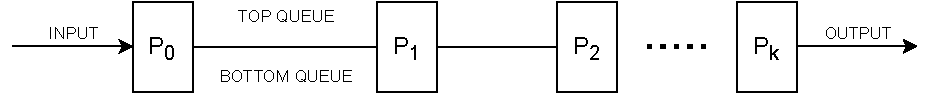
\includegraphics[scale=0.8]{pms_diagram.pdf}
            \caption{Diagram of the merge sorting pipeline.}
            \label{pms_diagram}
        \end{figure}

        The first process ($P_0$) serves as the input parser that loads the input values and sends them one by
        one to $P_1$. After parsing every input value, $P_0$ may exit. The rest of the processes
        ($P_i | 1\leq{}i\leq{}k$) work very similarly to each other. They all carry out two operations (\emph{receive}
        and \emph{merge})\footnote{Functions \texttt{receive()} and \texttt{merge()} in the implementation.} during each
        sorting cycle.

        Figure \ref{sequence_diagram} shows the lifetimes of the processes. The first process receives no messages,
        it only sends the input values to the second process. The rest of the processes must first wait until they
        receive the appropriate number of values and only then they may begin sorting. This is signified by the slight delay
        between receiving the first value and sending the first sorted value to the next process. Every process terminates
        after sorting $n$ values.

        \begin{figure}[h]
            \centering
            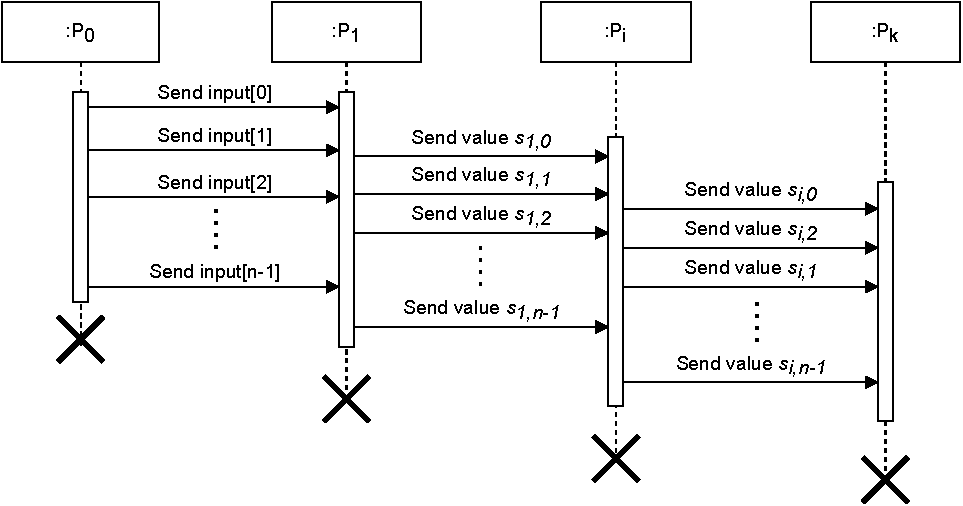
\includegraphics[scale=0.8]{sequence_diagram.pdf}
            \caption{The sequence diagram of the pipeline merge sort implementation. The symbol $s_{i,j}$ represents
            the $j$-th sorted value sent by process $i$.}
            \label{sequence_diagram}
        \end{figure}

        \subsection*{Receive}
        Every $Pi$ manages its input queues,
        so that they are assigned the correct number of incoming values sent from the previous process. This number, $q$, is
        governed by the rank of the current process, such that $q = 2^{i-1}$. The incoming values are first assigned to the
        top queue up until $q$ number of values is reached, after which the queue is switched and the incoming values are
        assigned to the bottom queue. After every $q$-th value, the queue is switched again.

        \subsection*{Merge}
        This operation sorts the values contained in the input queues by merge sorting. The process merges the first value
        only after its top queue contains $q$ values and the bottom contains at least one. One full merge cycle is completed
        after taking $q$ number of values from both input queues (i.e. $2q$ values in total). The process compares the first
        values of the input queues and the lower value is sent to the next process $P_{i+1}$. Each process must take
        at most $q$ number of values from each of its input queues via comparison. Otherwise the remaining values, until $2q$,
        are taken from the other queue regardless of those values' relation to any other values in the input queue.
        After a full merge cycle, the process restarts the merge cycle and repeats it until all input values have been merged.
        The last process in the pipeline is only different in that its output value is not sent to the next process, but rather
        to the output data structure (or, as in the case of this implementation, to the standard output stream).

        \section{Complexity and cost}
        The required number of processes is $p(n) = \log_{2}(n)+1$, where $n$ is the number of input values. The time complexity
        can be derived from the number of values needed by each process to begin sorting and the total number of inputs.
        Process $P_0$ requires $1$ input to start sorting and all remaining inputs will be processed in parallel with the rest
        of the processes. Every other process requires the top queue to be full and the bottom queue to contain at least one value.
        This means $2^{i-1} + 1$ steps before the $i$-th process may start sorting. Generalized to the $k$-th process in the pipeline,
        the following equation can be derived:
        \begin{equation}\label{eq:1}
            1 + \sum_{i=1}^{k}(2^{i-1}+1) = 2^{k} + k\,.
        \end{equation}
        However the last process needs an additional $n-1$ steps until all values are merged. This yields
        \begin{equation}\label{eq:2}
            2^{k} + k + (n-1) = 2^{\log_{2}(n)} + \log_{2}(n) + (n-1)
        \end{equation}
        steps for completely sorting $n$ input values through the $k$-th process. The index $k$ was substituted for its formula
        on the right hand side of equation \ref{eq:2}. After simplifying the previous, we are left with
        \begin{equation}\label{eq:3}
            2n + \log_{2}(n) - 1\,.
        \end{equation}

        The cost of a parallel algorithm is defined as $c(n) = p(n) * t(n)$, where $p(n)$ is the number of required processes for $n$
        inputs, and $t(n)$ is the number of steps required for completing the algorithm with $n$ inputs. The process requirement is
        $\log_{2}(n)+1$, which may be notated as $O(\log_{2}(n))$. The time complexity was shown in equation \ref{eq:3},
        which may be notated as $O(n)$. Therefore the cost of the algorithm is
        \begin{equation}\label{eq:4}
            c(n) = O(\log_{2}(n)) * O(n) = O(nlog_{2}(n))\,.
        \end{equation}
        As shown in equation \ref{eq:4}, the algorithm is optimal.

        \section{Conclusion}
        The implemented pipeline merge sorting algorithm works well on 16 values. It however could easily be modified to accept
        an arbitrary number of inputs. The Open MPI library provided easily introducable message passing capabilities into the
        implementation.

\end{document}